\documentclass[11pt]{article}
\usepackage[czech]{babel}
\usepackage[utf8]{inputenc}
\usepackage[T1]{fontenc}
\usepackage{fullpage}
\usepackage{graphicx}
\renewcommand{\baselinestretch}{1.2}

\begin{document}
\section{Mechanické složení}
Konstrukce z Merkuru. Držák na sensor čáry vytištěn na 3D tiskárně. Držák na ultrazvukové sensory ze dřeva. Veškeré komponenty jsou k hlavní desce propojeny přes ploché nakrimpované kabely. Baterie připojena na svorkovnici, ze které vede kabel na spínač a následně do svorkovnice na hlavní desce. Hlavní deska s Arduinem je uchycena vzhůru nohama uprostřed robota pro lepší rozložení hmotnosti.

\section{Elektrická část}
Všechna propojení a připojení jsou na hlavní univerzální desce.
\begin{figure}[h]
	\centering
	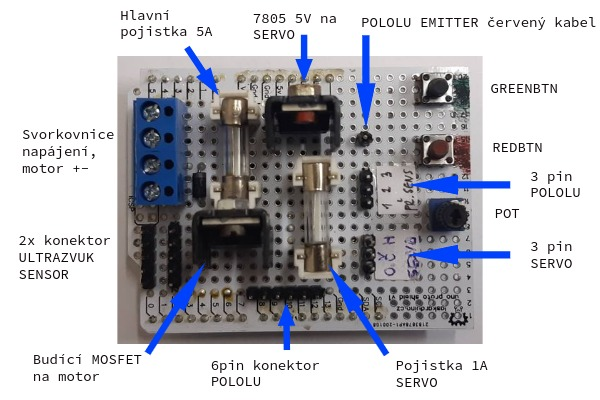
\includegraphics[scale=0.75]{deska.jpg}	
	\caption{Hlavní elektrická deska}
	\label{1}
\end{figure}
\subsection{Napájení}
Napájení z 7.5V Li-on baterie přes svorkovnici a spínač. Na hlavní desce se nachází 5A pojistka, přes kterou se toto napětí rozvádí do Pololu zemního sensoru, motoru a jako vstup na napájení Arduina (má vlastní stabilizátor, takže si s přebytkem napětí poradí). Také toto napětí jde do stabilizátoru 7805, který produkuje 5V pro napájení serva (Arduino by nestačilo).
\subsection{Ultrazvukové sensory}
Připojují se přes žílové kabely na hlavní desku na 2x 5 pin konektory. Pro debug je napsána funkce \texttt{debugSonic}.
\subsection{Pololu zemní sensory}
Připojuje se přes tři žílové kabely. Velký žílový kabel je pro šest snímacích sensorů, které se připojují na 6 pin konektor 8-13. Malý žílový kabel je napájecí kabel, kde 1 je zem, 2 je 5V a 3 7.5V. Poslední červený kabel je pro jakýsi emittor.
\subsection{Servo}
Připojuje se na hlavní desku do 3 pin konektoru, který je popsán O (oranžová), Č (červená) a H (hnědá). Napájení 5V z vlastního stabilizátoru s pojistkou 1A.
\subsection{Motor}
Poháněcí motor se zapojuje do velké modré svorkovnice s označením M+ a M-. Napájení přímo 7.5V.

\section{Firmware}
Hlavní program \texttt{robot$\_$v5.1.ino} s knihovnami \texttt{debugs.h}, \texttt{tests.h}, \texttt{corecontrols.h} a \texttt{defines.h}.  

\end{document}
